\section{Problema 3: Biohazard}

\subsection{Presentaci\'on del problema}
%aca ponemos una interpretacion de lo que nos pide el enunciado y algunas aclaraciones de como vamos a encarar el problema.
Tenemos una cantidad $n$ de productos químicos que deseamos repartir en la menor cantidad de camiones posible, con la particularidad de que no se supere un umbral $M$ de peligrosidad, el cual tenemos definido para cada par de productos. Entonces, la peligrosidad para un camión $C$ está dada por
\begin{align*}
peligrosidadCamion(C) = \sum\limits_{\substack{p_i,p_j \in C \\ i < j}} peligrosidadEntreProductos(p_i,p_j)
\end{align*}
Resolveremos este problema usando un algoritmo de backtracking implementando podas para reducir el tiempo de cómputo.

\subsection{Resoluci\'on}
\subsubsection{Algoritmo}
%aca ponemos una descripcion de nuestro algoritmo, presentamos la variables las estructuras y decimos que hacemos.
Definimos la estructura Camión que usaremos como contenedor de los productos como
\begin{align*}
Camion \: es \: tupla<peligrosidad : nat, productos : conjunto(nat)>
\end{align*}
La clave está en la función de backtracking
\begin{align*}
bt(p : nat, camiones : vector<Camion>, mejorTemp : vector<Camion>, M : nat, n : nat)
\end{align*}
donde $p$ es el i-ésimo producto a repartir, $camiones$ es la vector actual de camiones (esto se pasa por referencia), $mejorTemp$ es la mejor solución hasta el momento (también se pasa por referencia), $M$ es la máxima peligrosidad permitida por camión, y $n$ es la cantidad de productos. $vector$ es la representación de la estructura de la STL de C++ $std::vector$, que a los efectos del pseudocódigo es un array redimensionable (cuando se supera el límite, se duplica su tamaño y se copian los elementos al nuevo array).
Dados los parámetros, lo que hace es lo siguiente: 
\begin{itemize}
\item Si ya se introdujeron todos los productos ($p = n$), salgo, pero si además la vector de camiones es más chica que la mejor solución temporal, la pongo como mejor solución.
\item Para cada camión en $camiones$, intento agregar a $p$. Si puedo hacerlo, llamo a \textit{bt(p+1,~camiones,~mejorTemp,~M,~n)}, e inmediatamente saco el producto del camión (ya que si se llegó acá es que terminó la rama de la llamada a $bt$, y en la próxima iteración del ciclo se intentará poner el producto en el próximo camión si hay alguno).
\item Si se llega acá significa que el producto no pudo meterse en ningún camión, entonces antes de agregar un camión nuevo y meter al producto ahí, calculamos si haciendo éso estamos empatando la cantidad de camiones que tiene nuestra mejor solución temporal. Si fuera así, no tiene sentido seguir. Si no, se agrega un camión con el $p$ adentro, se llama a \textit{bt(p+1,~camiones,~mejorTemp,~M,~n)}, e inmediatamente se saca al camión que habíamos agregado (ya que aquí ya terminamos de recorrer esa rama del árbol de backtracking)
\item Llegado acá, la función simplemente termina.
\end{itemize}
La primera llamada a la función $bt$ se hace con el producto $1$, $camiones$ tiene un camión con el producto $0$, y siendo $mejorTemp$ la solución trivial de $n$ camiones con un producto en cada uno.


\subsubsection{Pseudoc\'odigo}
%aca va el pseudocodigo del problema.
\begin{algorithm}[H]
\begin{algorithmic}[1]
\caption{bt(p : nat, camiones : vector$<$Camion$>$, mejorTemp : vector$<$Camion$>$, M : nat, n : nat)}
\IF {p $==$ n \AND camiones.size() $<$ mejorTemp.size()}
	\STATE mejorTemp $\leftarrow$ camiones
    \RETURN
\ENDIF
\IF {p $==$ n}
	\RETURN
\ENDIF
\FOR {j $\leftarrow$ 0 \TO j $\leftarrow$ camiones.size() $-$ 1}
	\STATE \textcolor{CadetBlue}{// agregarNoSuperaUmbral(p, camion, M) devuelve \textbf{true} si el producto $p$ puede agregarse al $camion$ sin superar el umbral de peligrosidad $M$}
	\IF {agregarNoSuperaUmbral(p, camiones$[$j$]$, M)} 
		\STATE peligrosidadPrevia $\leftarrow$ agregarProducto(p, camiones$[$j$]$) \textcolor{CadetBlue}{// Esto agrega el producto y devuelve la peligrosidad previa a agregar éste}
		\STATE bt(p $+$ 1, camiones, mejorTemp, M, n)
		\STATE sacarProducto(p, camiones$[$j$]$, peligrosidadPrevia) \textcolor{CadetBlue}{// Quita el producto del camión y pone la peligrosidad previa para evitar recalcularla}
	\ENDIF
\ENDFOR
\IF {camiones.size() $<$ mejorTemp.size() $-$ 1}
	\STATE camiones.push\_back(Camion(p))
	\STATE bt(p $+$ 1, camiones, mejorTemp, M, n)
	\STATE camiones.pop\_back()
\ENDIF
\RETURN
\end{algorithmic}
\end{algorithm}

\begin{algorithm}[H]
\begin{algorithmic}[1]
\caption{agregarNoSuperaUmbral(p : nat, camion : Camion, M : nat) : bool}
\STATE acumPeligrosidad $\leftarrow$ camion.peligrosidad
\FOR {\textbf{each} producto $\in$ camion.productos}
	\STATE acumPeligrosidad $+=$ peligrosidades$[$p$][$producto$]$ \textcolor{CadetBlue}{// $peligrosidades$ es una matriz de n x n con las peligrosidades para cada par de productos}
	\IF {acumPeligrosidad $>$ M}
		\RETURN \FALSE
	\ENDIF
\ENDFOR
\RETURN \TRUE
\end{algorithmic}
\end{algorithm}

\begin{algorithm}[H]
\begin{algorithmic}[1]
\caption{agregarProducto(p : nat, camion : Camion) : nat}
\STATE peligrosidadPrevia $\leftarrow$ camion.peligrosidad
\FOR {\textbf{each} producto $\in$ camion.productos}
	\STATE camion.peligrosidad $+=$ peligrosidades$[$p$][$producto$]$
\ENDFOR
\STATE camion.productos.insert(p);
\RETURN peligrosidadPrevia
\end{algorithmic}
\end{algorithm}

\begin{algorithm}[H]
\begin{algorithmic}[1]
\caption{sacarProducto(p : nat, camion : Camion, peligrosidadPrevia : nat)}
\STATE camion.productos.erase(p)
\STATE camion.peligrosidad $\leftarrow$ peligrosidadPrevia
\end{algorithmic}
\end{algorithm}


%\subsection{Demostraci\'on} %OPCIONAL
%aca va la demostracion formal del problema refiriendonos al pseudocodigo o redefiniendo variables (definir todas las cosas de las que vamos a hablar).

\subsection{An\'alisis de complejidad}
%aca decimos cuanto cuesta cada parte del algoritmo y damos un valor final de la complejidad del algoritmo, ej O(logn).
Empecemos analizando la complejidad temporal de peor caso de las funciones auxiliares que utiliza el algoritmo. Sea $n$ la cantidad de productos, y $M$ la máxima peligrosidad permitida en un camión:
\begin{itemize}
	\item \textbf{sacarProducto} es O(log $|$camion.productos$|$) pues lo único que hace es modificar un variable entera, lo cual es O(1), y borrar un elemento del conjunto de productos del camión, lo cual es O(log $|$camion.productos$|$) ya que estamos representando al set de la STL.
	\item \textbf{agregarProducto} es O($|$camion.productos$|$) ya que se suman las peligrosidades entre el producto pasado por parámetro y los que ya están en el camión, lo cual es O($|$camion.productos$|$), y se inserta en el conjunto de productos, lo cual es O(log $|$camion.productos$|$).
	\item \textbf{agregarNoSuperaUmbral} es similar a la anterior, hace un ciclo sobre los productos del camión, acumulando las peligrosidades y hace un chequeo entre enteros, en total es O($|$camion.productos$|$).
\end{itemize}
Para la complejidad de \textbf{bt} vamos a necesitar un análisis más detallado. La función es llamada con un camión ya con el primer producto adentro, entonces el segundo producto va a tener dos posibilidades: o entrar a ese camión, o ir en un camión aparte. En el peor caso, se va a llamar recursivamente a \textbf{bt} para ambas configuraciones. Es decir, si $i$ es la cantidad de productos sin repartir,  $k$ es la cantidad de camiones actual, y $c_j$ es la cantidad de productos en el j-ésimo camión:
\begin{align*}
T(i,k) = \left(\sum\limits_{\substack{j = 1}}^k O(c_j) + T(i-1,k)\right) + O(1) + T(i-1,k+1) + O(1)
\end{align*}
Dentro de la suma está la complejidad de cada iteración del ciclo que recorre los camiones, siempre haremos \textbf{agregarNoSuperaUmbral} que es $O(c_j)$ y en el peor caso se llama a \textbf{agregarProducto} (de nuevo $O(c_j)$) y hará la recursión con un producto menos; luego se hace \textbf{sacarProducto} que es $O(\log c_j)$. Como la suma de los productos de todos los camiones es la cantidad de productos ya repartidos, podemos acotar $\sum\limits_{\substack{j = 1}}^k c_j$ con $n-i$. Fuera de la sumatoria tenemos el costo de agregar un camión nuevo, llamar recursivamente con un producto menos y un camión más (con el elemento que le pusimos), y de sacar el camión agregado. Sacar y poner un camión en un array redimensionable tiene una complejidad amortizada de O(1). Entonces, queda:
\begin{align*}
T(i,k) &= O(n-i+1) + k \times T(i-1,k) + T(i-1,k+1)
\end{align*}
El problema de esta ecuación es que es difícil ver la complejidad con respecto a la cantidad $n$ de productos iniciales. Sabemos que nuestro algoritmo se comporta así: para el primer producto, solamente llama a \textbf{bt} una vez, ya que hay un solo camión, y por lo tanto una sola posibilidad; en cambio, para el segundo producto hay dos: o lo mete en el primer camión, o lo mete en uno nuevo; y ahora tenemos dos configuraciones para el producto 3, y cinco posibilidades. Sabemos que en todo momento no puede haber más camiones que productos ya repartidos, entonces podemos acotar $k$ inferiormente con $n-i$. Así, podemos definir:
\begin{align*}
T(i) &= O(n-i+1) + (n-i) \times T(i-1) + T(i-1) \text{ y entonces queda: } \\
T(i) &= O(n-i+1) + (n-i+1) \times T(i-1) \\
\text{ Evaluando en n: } \\
T(n) &= O(1) + T(n-1) \\
T(n) &= O(1) + O(2) + 2 \times T(n-2) \\
T(n) &= O(1) + O(2) + 2 \times O(3) + 2 \times 3 \times T(n-3) \\
T(n) &= O(1) + O(2) + O(2 \times 3) + O(2 \times 3 \times 4) + 2 \times 3 \times 4 \times T(n-4) \\
\vdots \\
T(n) &= O\left(\sum\limits_{\substack{i = 1}}^n i!\right) + O(n!)
\end{align*}
Por lo tanto, la complejidad temporal de peor caso es $O\left(\sum\limits_{\substack{i = 1}}^n i!\right)$.

\subsection{Tests de complejidad}
%aca van los graficos y todos los testeos que hagamos para probar que en la practica el algoritmo cumple la complejidad que propusimos en el punto anterior
Testearemos instancias aleatorias con cantidad de productos en $[2,...,15]$. Los tiempos para cada valor $n$ de productos se calculan como el promedio del tiempo de las instancias, donde a su vez el tiempo para cada instancia será el mínimo de varias ejecuciones del algoritmo, para mejorar la precisión. Para los casos sin podas o con podas malas, se tomaron pocas instancias ya que el tiempo de ejecución era astronómicamente alto (se tomaron 5 instancias, con 2 cálculos para el mínimo en cada una). Para los demás casos, se tomaron 500 instancias con 10 cálculos de mínimo para cada una.

En la sección anterior dijimos que la complejidad del algoritmo sin podas es $O\left(\sum\limits_{\substack{i = 1}}^n i!\right)$. Hicimos tests de medición de tiempo para corroborar esto. Notemos que 
\begin{align*}
O\left(\sum\limits_{\substack{i = 1}}^n i!\right) \in O(n \times n!)
\end{align*}
Por otro lado, por propiedades del logaritmo, 
\begin{align*}
ln(n \times n!) &= ln(n) + ln(n!)
\end{align*}
También sabemos que por la aproximación de Stirling del factorial, 
\begin{align*}
ln(n!) &= n \times ln(n) - n + O(ln(n))
\end{align*}
Por lo tanto, a partir de algún $n$ vale que 
\begin{align*}
ln(n \times n!) \approx ln(n) + n \times ln(n) - n = (n+1) ln(n) - n
\end{align*}
En el próximo gráfico ploteamos, para $n$ $=$ cantidad de productos, $t_n$ $=$ tiempo promedio para n productos, la función $f(n) = \frac{ln(t_n)}{(n+1) ln(n) - n}$ lo cual a partir de algún $n$ debería ser constante. En efecto:

\begin{figure}[H]
	\begin{minipage}[t]{\linewidth}
		\centering
		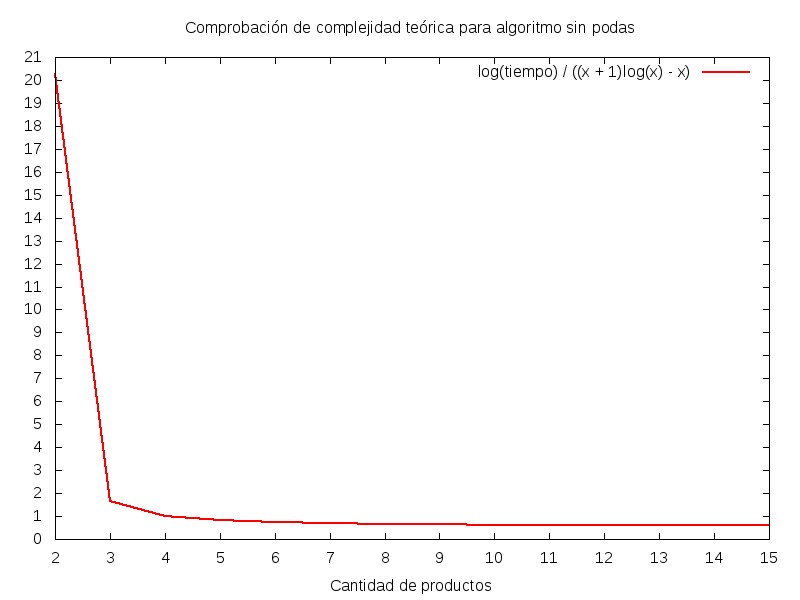
\includegraphics[width=\textwidth]{complejidad.jpg}
		%\caption{Con colisión total}
		\label{fig:p3_complejidad}
	\end{minipage}
\end{figure}

Analicemos ahora cómo se comporta el algoritmo con las siguientes podas: 
\begin{enumerate}
\item Sabiendo que en la rama en la que estoy tenemos $C-1$ camiones, donde $C$ es la cantidad de camiones de la mejor solución hasta el momento, al insertar exitosamente un producto en alguno de los camiones, va a chequear --antes de llamar a la recursión-- si el resto de los productos pueden entrar en algún camión. Si algún producto no puede entrar en ningún camión, eso implica que necesitamos al menos un camión más, lo cual empata a la mejor solución, es entonces donde se poda esta rama que no llevará a nada mejor. El problema de esta cota es que pueden estar recalculándose múltiples veces si un producto $x$ entra en un camión $y$, lo cual puede ser un problema porque cada vez que se ejecuta esta poda se hacen $O(n^2)$ comparaciones de peligrosidades.
\item Esta cota también se activa al estar en $C-1$ camiones, y es más simple y rápida que la anterior: si llegamos al punto donde tenemos que agregar un camión, salimos, porque empatamos a la mejor solución y no sirve toda esa rama.
\end{enumerate}

Si vemos los tiempos de las tres configuraciones, tenemos:
\begin{figure}[H]
	\begin{minipage}[t]{\linewidth}
		\centering
		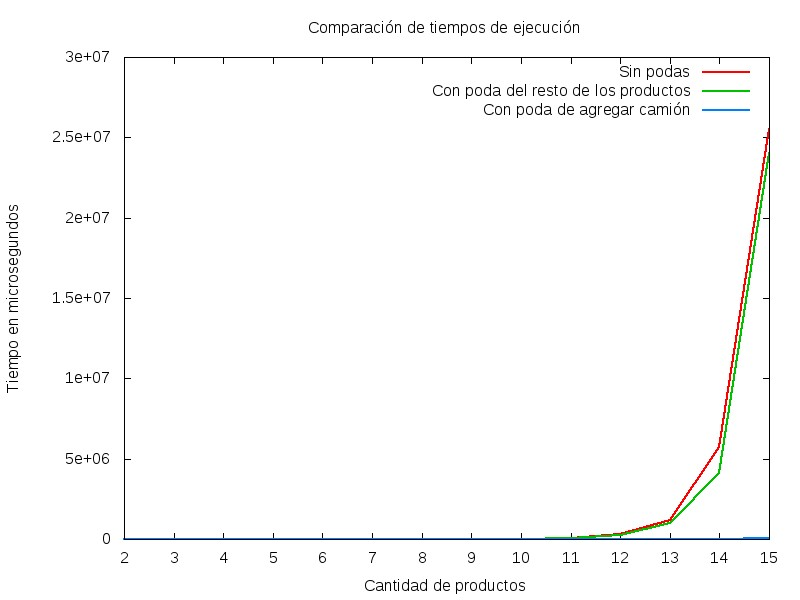
\includegraphics[width=\textwidth]{comparacion_tiempos_podas.jpg}
		%\caption{Con colisión total}
		\label{fig:p3_comparacion_3_configuraciones}
	\end{minipage}
\end{figure}

Como vemos en la figura, sólamente podar por resto de los productos no mejora demasiado el costo temporal, pero tampoco lo empeora. Por otro lado, casi no se ve la poda de agregar camión, cuya efectividad es relativamente buena. Cabría preguntarse si esta segunda poda obtiene una complejidad mejor que $O(n \times n!)$. Lamentablemente, no es así, como podemos ver en el siguiente gráfico:

\begin{figure}[H]
	\begin{minipage}[t]{\linewidth}
		\centering
		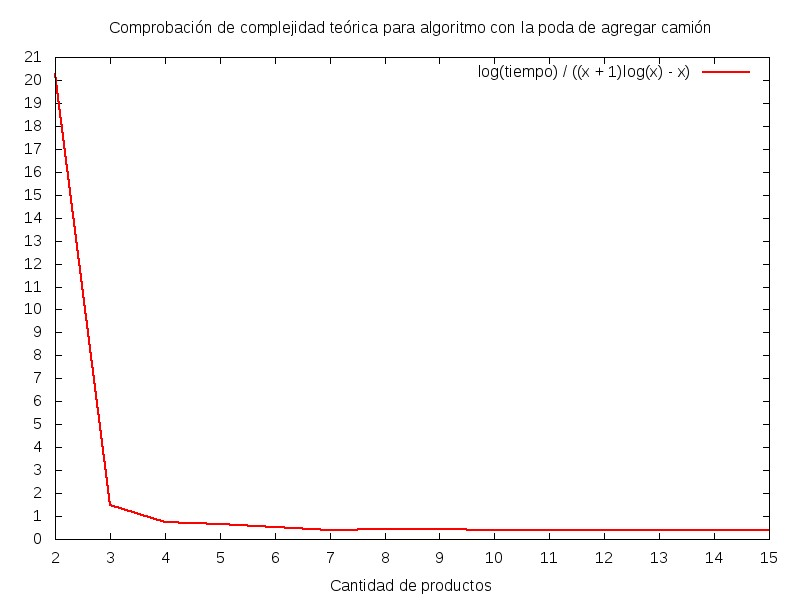
\includegraphics[width=\textwidth]{complejidad_con_poda_camion.jpg}
		%\caption{Con colisión total}
		\label{fig:p3_complejidad_con_poda_camion}
	\end{minipage}
\end{figure}

A pesar de esto, para valores bajos de $n$ es una excelente poda. Por último, podemos evaluar qué ocurre si usamos ambas podas. Comparémoslas:

\begin{figure}[H]
	\begin{minipage}[t]{\linewidth}
		\centering
		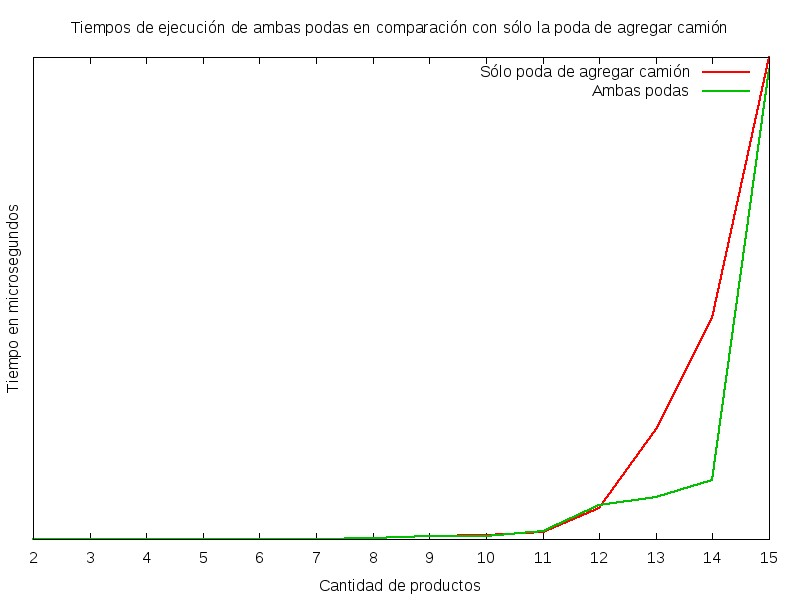
\includegraphics[width=\textwidth]{comparacion_poda_camion_con_ambas_podas.jpg}
		%\caption{Con colisión total}
		\label{fig:p3_comparacion_poda_camion_con_ambas_podas}
	\end{minipage}
\end{figure}

Logramos mejorar aún más el tiempo de ejecución para valores bajos, aunque rápidamente alcanza a la poda anterior.
